\section[The ms+seqgen Approach]{The \code{ms+seqgen} Approach}
\label{sec:msseqgen}
\addcontentsline{toc}{section}{\thesection. The \code{ms+seqgen}\ Approach}

\pkg{Phyclust} incorporates two popular open source \proglang{C} programs:
\pkg{ms} \citep{Hudson2002} and \pkg{seq-gen} \citep{Rambaut1997}.
The original source code and documentation are available on the authors'
original websites, or the mirror on phyloclustering website at
\url{http://thirteen-01.stat.iastate.edu/snoweye/phyclust/}.

The \pkg{ms} documentation demonstrates how to use \pkg{ms}
to generate coalescent trees, followed by sequence generation using \pkg{seq-gen},
the popular \code{ms+seqgen} approach for simulating molecular data.
I have edited the source code slightly to make these commands available through new \proglang{R} functions \code{ms()} and \code{seqgen()}.
This solution eases the burden on the user, bypassing the need to compile both programs.
Moreover, combining these functions with the \code{phyclust()} function produces a
\code{ms+seqgen+phyclust} approach 
 for simulation and bootstrap studies (see Section~\ref{sec:msseqgenphyclust}).




\subsection[Using the ms() function to generate trees]{Using the \code{ms()} function to generate trees}
\label{sec:ms}
\addcontentsline{toc}{subsection}{\thesubsection. Using the \code{ms()}\ function to generate trees}

Almost all command line options of program \pkg{ms} are available
through option \code{opts} in \code{ms()}.
Call the function without arguments to see all the options.
\begin{Code}
> ms()
> ?ms
\end{Code}

The following example generates a coalescent tree (\pkg{ms} option \code{-T})
with 3 leaves (\code{nsam = 3})
and population growth rate 0.1
(\code{-G 0.1}). Function \code{ms()} returns \pkg{ms} text output
stored in an array, one line per element.
The third line contains the tree in NEWICK format, which can
be read by the \code{read.tree()} function in the \pkg{ape} package
\citep{Paradis2004}.
Function \code{read.tree()} returns an object of class \code{phylo},
which can be drawn by function \code{plot()} or \code{plot.phylo()}
of the \pkg{ape} package.
\begin{Code}
> set.seed(1234)
> (ret.ms <- ms(nsam = 3, opts = "-T -G 0.1"))
ms 3 1 -T -G 0.1 
//
(s1: 0.568774938583,(s2: 0.355949461460,s3: 0.355949461460): 0.212825477123);
> (tree.anc <- read.tree(text = ret.ms[3]))

Phylogenetic tree with 3 tips and 2 internal nodes.

Tip labels:
[1] "s1" "s2" "s3"

Rooted; includes branch lengths.
> tree.anc$tip.label <- paste("a", 1:3, sep = "")
> plot(tree.anc, type = "c")
> axisPhylo()
\end{Code}
\begin{figure}[h]
%pdf("f-ms.pdf", width = 5, height = 4)
%plot(tree.anc, type = "c")
%axisPhylo()
%dev.off()
\begin{center}
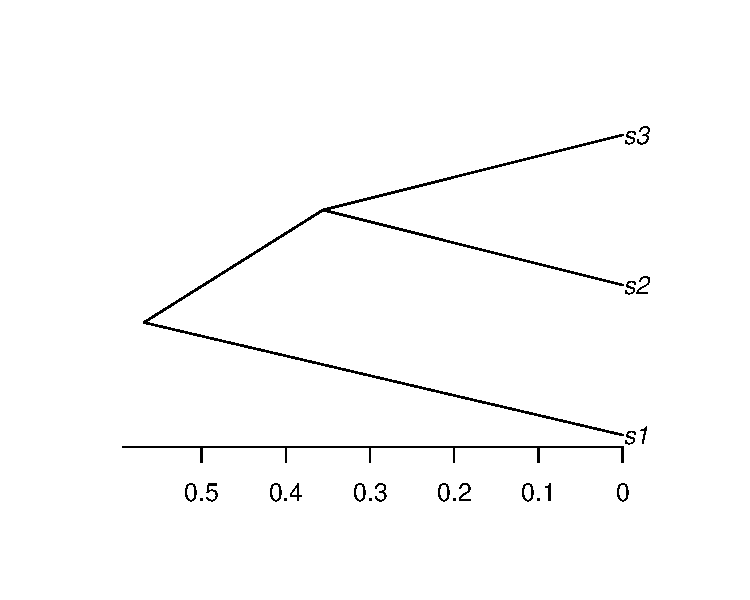
\includegraphics[width=5.0in]{./phyclust-include/f-ms}
\caption{A diagram of a simple coalescent tree.}
\label{fig:ms}
\end{center}
\end{figure}




\subsection[Using the seqgen() function to generate sequences]{Using the \code{seqgen()} function to generate sequences}
\label{sec:seqgen}
\addcontentsline{toc}{subsection}{\thesubsection. Using the \code{seqgen()}\ function to generate sequences}

Almost all options of the command line program \pkg{seq-gen} are available from within \proglang{R} via
the option \code{opts} in the \code{seqgen()} function.
Call the function without arguments to see the options.
\begin{Code}
> seqgen()
> ?seqgen
\end{Code}

The \code{seqgen()} function requires a rooted tree in NEWICK format or an object of class \code{phylo}.
In the following, we demonstrate the \code{ms+seqgen} approach
to generate sequences. The result is a character
vector of class {\color{red} \code{seqgen}}, which contains 5 sequences, 
each of 40 bases (\pkg{seq-gen} option \code{-l40}). The option \code{-mHKY} specifies the HKY85
model of evolution \citep{Hasegawa1985}.
Without further options, HKY85 is equivalent to the JC69 model \citep{Jukes1969}.
\begin{Code}
> set.seed(123)
> ret.ms <- ms(nsam = 5, nreps = 1, opts = "-T")
> tree.anc <- read.tree(text = ret.ms[3])
> set.seed(123)
> seqgen(opts = "-mHKY -l40", newick.tree = ret.ms[3])
 5 40
s1        CTCTCATTGGACGCACACTTTAGGGGGGGATTGCACTGCA
s5        CTCTCTCTGGACGCACACTTTAAGGGGGGATTGAACTACA
s2        CTCTTCGGGCTCGGATAAGTTTGGAGGGTTGTTCTCTACA
s3        CTCTGAGTGCTCGGATTAGTTAGGGGGAATGACGTCTACA
s4        CTCTTATCTCTCGGATAAGTTGGGGGTGATGGCTTTTACA
> set.seed(123)
> (ret.seq <- seqgen(opts = "-mHKY -l40", rooted.tree = tree.anc))
 5 40
s1        CTCTCATTGGACGCACACTTTAGGGGGGGATTGCACTGCA
s5        CTCTCTCTGGACGCACACTTTAAGGGGGGATTGAACTACA
s2        CTCTTCGGGCTCGGATAAGTTTGGAGGGTTGTTCTCTACA
s3        CTCTGAGTGCTCGGATTAGTTAGGGGGAATGACGTCTACA
s4        CTCTTATCTCTCGGATAAGTTGGGGGTGATGGCTTTTACA
> str(ret.seq)
Class 'seqgen'  chr [1:6] " 5 40" "s1        CTCTCATTGGACGCACACTTTAGGGGGG ...
\end{Code}

The \code{seqgen()} function need not take in a tree from \code{ms()},
but \code{ms()} provides options to construct trees of
different shapes using coalescent theory.
Also, you can provide \code{seqgen()} with an ancestral sequence that is then evolved along the given tree (see Section~\ref{sec:ancestral}).




\subsection[Inputing an ancestral sequence to ms+seqgen]{Inputing an ancestral sequence to \code{ms+seqgen}}
\label{sec:ancestral}
\addcontentsline{toc}{subsection}{\thesubsection. Inputing an ancestral sequence to \code{ms+seqgen} \vspace{-0.3cm}}

\pkg{Phyclust} provides two functions \code{gen.seq.HKY()} and
\code{gen.seq.SNP()} to implement the \code{ms+seqgen}
approach under wide-ranging parameter choices. A rooted tree is required and an
ancestral sequence is an option.

The following example generates a tree and provides an ancestral
sequence. Function \code{seqgen()} will use
parameters $\kappa$ (\code{kappa}) and
$\pi_{A}, \pi_{G}, \pi_{C}, \pi_{T}$ (\code{pi.HKY})
to evolve the ancestral sequence (\code{anc.HKY}) down the tree.
The function \code{read.seqgen()} reads the \code{seqgen()}
object and returns a new dataset of class \code{seq.data}
for use by the function \code{phyclust()} (see Section~\ref{sec:phyclust}).
\begin{Code}
> # Generate a tree
> set.seed(1234)
> ret.ms <- ms(nsam = 5, nreps = 1, opts = "-T")
> tree.ms <- read.tree(text = ret.ms[3])
> 
> # Generate nucleotide sequences
> (anc.HKY <- rep(0:3, 3))
 [1] 0 1 2 3 0 1 2 3 0 1 2 3
> paste(nid2code(anc.HKY, lower.case = FALSE), collapse = "")
[1] "AGCTAGCTAGCT"
> pi.HKY <- c(0.2, 0.2, 0.3, 0.3)
> kappa <- 1.1
> L <- length(anc.HKY)
> set.seed(1234)
> (HKY.1 <- gen.seq.HKY(tree.ms, pi.HKY, kappa, L, anc.seq = anc.HKY))
 5 12
s1        AGCTTGACCGGC
s3        AGCTTCACCGGT
s2        ACCTCGCTAGCT
s4        ACGACGCTCGCT
s5        CCTACGCTAGCT
> (ret <- read.seqgen(HKY.1))
code.type: NUCLEOTIDE, n.seq: 5, seq.len: 12.
\end{Code}

Function \code{gen.seq.HKY()} may be a good example
for advanced users wanting to simulate more complex evolutionary processes, such as recombination,
migration and island models. It passes an option \code{input} to
\code{seqgen()}, which in this case is used to pass the ancestral sequence, but could be used to pass other
options available in the \pkg{seq-gen} program.
The option \code{input} takes in a character vector (including the tree)
where each element contains one \pkg{seq-gen} option.
Function \code{seqgen()} writes these options to
a temporary file, which is later communicated to \pkg{seq-gen}.
\begin{Code}
### Partial source code of gen.seq.HKY().
        L <- length(anc.seq)
        mu <- paste(nid2code(anc.seq, lower.case = FALSE), collapse = "")
        seqname <- paste("Ancestor  ", collapse = "")
        input <- c(paste(" 1", length(anc.seq), sep = " "), paste(seqname, 
            mu, sep = ""), 1, write.tree(rooted.tree, digits = 12))
        opts <- paste("-mHKY", " -t", ts.tv, " -f", paste(pi[c(1, 
            3, 2, 4)], collapse = ","), " -l", L, " -s", rate.scale, 
            " -u", ttips + 1, " -k1", " -q", sep = "")
        ret <- seqgen(opts, input = input)

### Partial source code of seqgen().
        if (!is.null(newick.tree)) {
            write(newick.tree, file = temp.file.ms, sep = "")
        }
        else if (!is.null(input)) {
            write(input, file = temp.file.ms, sep = "\n")
        }
        else {
            stop("A newick or rooted/phylo tree is required.")
        }
\end{Code}

